%Vorlage fuer Thesen an der FFHS
\documentclass{ksgr_style}
\usepackage[utf8]{inputenc}
\usepackage{float} % Hold figures and tables on place
\usepackage{longtable}
\usepackage{multicol}
\usepackage{paracol}

\usepackage{booktabs}
\usepackage{multirow}
\usepackage[table,xcdraw]{xcolor}
% Beamer presentation requires \usepackage{colortbl} instead of \usepackage[table,xcdraw]{xcolor}
\usepackage{lscape}
\usepackage[toc, xindy]{glossaries}
\usepackage{textcomp}
\usepackage{rotating}
\usepackage{pdflscape}

\usepackage{enumitem,hyperref}


\usepackage[explicit]{titlesec}
\usepackage{calc,pifont,eurosym,amsmath,wasysym,amssymb,amsfonts}

\hypersetup{colorlinks=true,allcolors=blue,pdftitle=KSGR KIS Phoenix JBoss Patch Dokumentation,pdfauthor=Michael Graber (gramic)}

%! Author = itgramic
%! Date = 09.10.23

% Preamble
%\makeglossaries
\makenoidxglossaries
\newglossaryentry{JBoss}
{
        name=JBoss,
        description={JBoss ist ein Applikationsserver für \Gls{Java} Anwendungen, die von Red Hat aufgekauft wurde.
        JBoss gilt als Standardserver für Java EE Anwendungen\cite{U4ZJDNI2}.}
}
\newglossaryentry{Java}
{
        name=Java,
        description={Java ist eine Hochsprache die 1995 von Sun Microsystems veröffentlicht wurde.
Dank der JVM läuft Java auf sehr vielen Plattformen\cite{6H25Z3UI}.}
}
\newglossaryentry{Ivanti}
{
        name=Ivanti,
        description={Das KSGR nutzt die Ivanti AppSense\cite{LPHK6T9X, 8CHLH32N} für die Verteilung von Software und dem Installieren von Patches.}
}
\newglossaryentry{RDP}
{
        name=RDP,
        description={Microsofts Protokoll für die Übertragung von Bildschirm- und Peripheriedaten von einem Remote-Rechner zu übertragen\cite{9PJHPCRS}.}
}


% Fortlaufende Nummerierung
\usepackage{listings}
\usepackage{csquotes}

% ASCII Folder Diagramm
\usepackage{dirtree}
%\usepackage{forest}

\usepackage[]{mdframed}

% Hyperref
\usepackage{hyperref}

% Bibliography Packages
\usepackage[style=numeric,backend=biber,sortlocale=de_DE,bibencoding=utf8,sorting=nty,minbibnames=1,maxbibnames=6,autopunct=true,natbib=true,hyperref=false,doi=false,isbn=false,url=false,eprint=false]{biblatex}
\DeclareLanguageMapping{american}{american-apa}
\addbibresource{source/ksgr_kis_phoenix_jboss_patch.bib}

\geometry{
   left=2.3cm,
   right=2.3cm,
   top=2.13cm,
   bottom=2cm,
   textwidth=8cm,
   marginpar=3cm}

% set listing designs
%New colors defined below
\definecolor{codegreen}{rgb}{0,0.6,0}
\definecolor{codegray}{rgb}{0.5,0.5,0.5}
\definecolor{codepurple}{rgb}{0.58,0,0.82}
\definecolor{backcolour}{rgb}{0.95,0.95,0.92}

%Code listing style named "mystyle"
\lstdefinestyle{gra_codestyle}{
  backgroundcolor=\color{lightgray}, commentstyle=\color{codegreen},
  keywordstyle=\color{magenta},
  numberstyle=\tiny\color{codegray},
  stringstyle=\color{codepurple},
  basicstyle=\ttfamily\footnotesize,
  breakatwhitespace=false,
  breaklines=true,
  captionpos=b,
  keepspaces=true,
  numbers=left,
  numbersep=5pt,
  showspaces=false,
  showstringspaces=false,
  showtabs=false,
  tabsize=2
}


\fancyhf{}% Clear all headers/footers
\fancypagestyle{headings}{\fancyhf{}
  \fancyfoot[R]{\fontsize{7.5pt}{13.8ptpt} \raggedleft\selectfont\sffamily\bfseries\color[HTML]{000000}\thepage{}}
  \fancyfoot[L]{\fontsize{7.5pt}{13.8ptpt} \raggedleft\selectfont\sffamily\bfseries\color[HTML]{000000}© Kantonsspital Graubünden | KIS Phoenix - JBoss Patch}
  \renewcommand\headrulewidth{0pt}
  \renewcommand\footrulewidth{0pt}
  \renewcommand\thepage{\arabic{page}}
}
\fancypagestyle{FirstPage}{\fancyhf{}
  \fancyhead[L]{}
  \fancyfoot[L]{}
  \renewcommand\headrulewidth{0pt}
  \renewcommand\footrulewidth{0pt}
  \renewcommand\thepage{\arabic{page}}
  \fancyhead[L]{
\includegraphics{source/main/ksgr}}
  \fancyhead[C]{\fontsize{7.5pt}{0ptpt} \raggedleft\selectfont\sffamily\bfseries\color[HTML]{000000}\makebox[32em][l]{Kantonsspital Graubünden} \\ \makebox[32em][l]{Departement ICT} \\ \makebox[32em][l]{\textbf{Data Center}} \\ \makebox[32em][l]{www.ksgr.ch} \\}
  \fancyhead[R]{\fontsize{7.5pt}{0ptpt} \raggedleft\selectfont\sffamily\bfseries\color[HTML]{000000}\makebox[8em][l]{\textbf{Michael}} \\ \makebox[8em][l]{\textbf{Graber}} \\ \makebox[8em][l]{Datenbank Administrator} \\ \makebox[8em][l]{michael.graber@ksgr.ch} \\ \makebox[8em][l]{+41 81 256 68 25} \\}
}
%    % Headings

\titleformat{\chapter}[block]{\filright\normalfont\normalsize\normalcolor\fontsize{11.5pt}{13.8pt}\selectfont\rmfamily\bfseries\color[HTML]{C60821}}{{\fontsize{12pt}{14.400001pt}\selectfont \makebox[2.5cm][l]{\thechapter}}}{0pt}{#1}[]
\titlespacing*{\chapter}{0pt}{0.847cm plus 0.1694cm minus 0.0847cm}{0.212cm plus 0.0424cm minus 0.0212cm}

\titleformat{\section}[block]{\filright\normalfont\normalsize\normalcolor\fontsize{11.5pt}{13.8pt}\selectfont\rmfamily\bfseries\color[HTML]{000000}}{{\fontsize{11pt}{14.400001pt}\selectfont \makebox[2.5cm][l]{\thesection}}}{0pt}{#1}[]
\titlespacing*{\section}{0pt}{0.847cm plus 0.1694cm minus 0.0847cm}{0.212cm plus 0.0424cm minus 0.0212cm}
\titleformat{\subsection}[block]{\filright\normalfont\normalsize\normalcolor\fontsize{10pt}{13.8pt}\selectfont\rmfamily\bfseries\color[HTML]{000000}}{{\fontsize{11pt}{14.400001pt}\selectfont \makebox[2.5cm][l]{\thesubsection}}}{0pt}{#1}[]
\titlespacing*{\subsection}{0pt}{0.847cm plus 0.1694cm minus 0.0847cm}{0.212cm plus 0.0424cm minus 0.0212cm}
\titleformat{\subsubsection}[block]{\filright\normalfont\normalsize\normalcolor\fontsize{10pt}{13.8pt}\selectfont\rmfamily\bfseries\color[HTML]{000000}}{{\fontsize{11pt}{14.400001pt}\selectfont \makebox[2.5cm][l]{\thesubsubsection}}}{0pt}{#1}[]
\titlespacing*{\subsubsection}{0pt}{0.847cm plus 0.1694cm minus 0.0847cm}{0.212cm plus 0.0424cm minus 0.0212cm}
\titleformat{\subsubsection}[block]{\filright\normalfont\normalsize\normalcolor\fontsize{10pt}{13.8pt}\selectfont\rmfamily\bfseries\color[HTML]{000000}}{{\fontsize{11pt}{14.400001pt}\selectfont \makebox[2.5cm][l]{\thesubsubsection}}}{0pt}{#1}[]
\titlespacing*{\subsubsection}{0pt}{0.847cm plus 0.1694cm minus 0.0847cm}{0.212cm plus 0.0424cm minus 0.0212cm}
\titleformat{\paragraph}[block]{\filright\normalfont\normalsize\normalcolor\fontsize{10pt}{13.8pt}\selectfont\rmfamily\bfseries\color[HTML]{000000}}{{\fontsize{11pt}{14.400001pt}\selectfont \makebox[2.5cm][l]{\theparagraph}}}{0pt}{#1}[]
\titlespacing*{\paragraph}{0pt}{0.847cm plus 0.1694cm minus 0.0847cm}{0.212cm plus 0.0424cm minus 0.0212cm}
\titleformat{\subparagraph}[block]{\filright\normalfont\normalsize\normalcolor\fontsize{10pt}{13.8pt}\selectfont\rmfamily\bfseries\color[HTML]{000000}}{{\fontsize{11pt}{14.400001pt}\selectfont \makebox[2.5cm][l]{\thesubparagraph}}}{0pt}{#1}[]
\titlespacing*{\subparagraph}{0pt}{0.847cm plus 0.1694cm minus 0.0847cm}{0.212cm plus 0.0424cm minus 0.0212cm}

\begin{document}
    \toptitel{Windows Patchday}
    \dokuemnttitel{KIS Phoenix - JBoss Patch}
    \datum{24.11.2023}
    \maketitle
    \clearpage
    \thispagestyle{fancy}
    \begin{managementsummary}
        \begin{flushleft}
            Dokumentiert wie die \Gls{JBoss}-Applikationsserver des KIS Phoenixs sowohl für das Test- als Produktivsystem gepatched werden können und welche Schritte dazu benötigt werden.
        \end{flushleft}
        \begin{flushleft}
            Es wird also auf die richtige Reihenfolge der stopps der Services und Server-Reboots eingegangen und wie man die Applikation im Anschluss testen kann.
        \end{flushleft}
    \end{managementsummary}
    \thispagestyle{fancy}
    \pagestyle{headings}
    {
        \hypersetup{hidelinks}
        \tableofcontents
    }
    \pagestyle{headings}
    \thispagestyle{fancy}
    %! Author = itgramic
%! Date = 03.10.23

% Preamble
\begin{abkuerzungen}[MUSTER] % Das Muster dient zur Bestimmung der Einrueckungstiefe
    \item[ICT] information and communications technology
    \item[KSGR] Kantonsspital Graubünden
    \item[KIS] Klinisches Informationssystem
    \item[\gls{JBoss}] JavaBean Open Source Software Application Sever
    \item{JVM} \Gls{Java} Virtual Machine
\end{abkuerzungen}
    \thispagestyle{fancy}
    \startThesis % Befehl muss vor dem ersten chapter stehen (Seitennummerierung!)
    \clearpage
    %! Author = itgramic
%! Date = 24.11.23

% Preamble
\chapter{Einführung}
\begin{flushleft}
    Im Rahmen des von Microsoft indizierten Patchdays, bei dem Microsoft alle 2 Monate einen Patch veröffentlicht, müssen auch die \Gls{JBoss}-Server des KIS Phoenix angefasst werden.
    Die Server werden dabei von \Gls{Ivanti} mit den Patches betankt, so das man nur noch einen Reboot durchführen und nicht noch erst die Patches herunterladen muss..
\end{flushleft}
\begin{flushleft}
    Das KIS Phoenix verfügt dabei über 4 JBoss-Server, 2 für die Testsysteme resp.
    das Demosytsem und 2 für das produktive System.
    \begin{figure}[H]
        \centering
        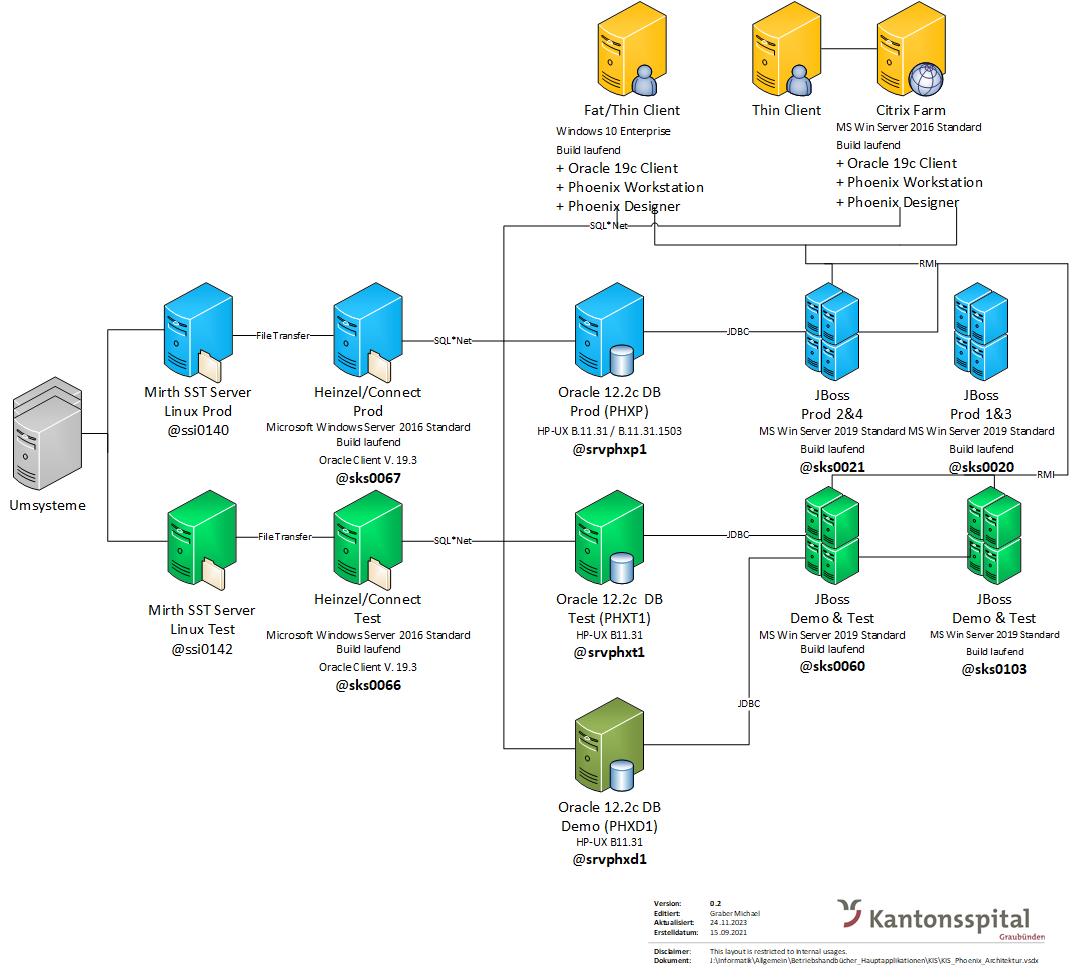
\includegraphics[width=1\linewidth]{source/introduction/KIS_Phoenix_Architektur}
        \caption{Architektur KIS Phoenix\cite{KFDFYH5H}}
        \label{fig:architektur-kis-phoenix}
    \end{figure}
\end{flushleft}
\begin{flushleft}
    Das Test1 und Demosystem hat je einen JBoss-Node auf einer Seite, das Test2 hat nur einen Node auf einem Server.
    Das Produktivsystem hat je Site zwei Nodes, also insgesamt vier Nodes.
\end{flushleft}
\begin{flushleft}
    Die Verzeichnisstruktur sieht dabei wie folgt aus:

%    \dirtree{%
%    .1 spam.
%    .2 ham.
%    .2 eggs.
%    .3 more spam.
%    .3 dead parrots.
%    }

%    \dirtree{%
%    .1 Laufwerk.
%    .2 {phoenix\_server\_system\_version}.
%    .3 node.
%    .4 standalone.
%    .5 log.
%    .6 server.log.
%    }

%    \dirtree{%
%
%    .1 spam.
%    .2 ham.
%    .2 eggs.
%    .3 more spam.
%    .3 dead parrots.
%%    .4 potatoes.
%    }

    \dirtree{%
        .1 /.
        .2 laufwerk.
        .3 phoenix-server-<system>-<version>.
        .4 <node>.
        .5 standalone.
        .6 log.
        .7 server.log.
    }

    \begin{mdframed}
    Meistens existieren pro Node die Verzeichnisse meherer Versionen, üblicherweise immer die der aktuellen und vorangehenden Version.\\Daher aufpassen in welchem Verzeichnis man ist!
    \end{mdframed}

    Auf jedem Server wurde zudem \textit{baretail.exe} installiert, ein Logging-Tool welches eine Echtzeitüberwachung der Logs ermöglicht.
    Leider ist es nicht auf jedem Server gleich installiert sondern individuell.

    Die genaue Konfiguration sieht wie folgt aus:
\end{flushleft}
    % Please add the following required packages to your document preamble:
    % \usepackage{booktabs}
    % \usepackage{graphicx}
    % \usepackage{lscape}
    \begin{landscape}
    \begin{table}[]
    \centering
    \resizebox{\columnwidth}{!}{%
    \begin{tabular}{@{}lccccccccccc@{}}
    \toprule
    \textbf{Typ}                                                     & \textbf{Applikationsserver} & \textbf{}                & \textbf{}                & \textbf{}                & \multicolumn{5}{c}{}                                                                                                                      & \multicolumn{2}{c}{\textbf{Schnittstellenserver}} \\ \midrule
    \textbf{\begin{tabular}[c]{@{}l@{}}Systeme\\ Rolle\end{tabular}} & \multicolumn{2}{c}{\textbf{Produktion}}                & \multicolumn{2}{c}{\textbf{Produktion}}             & \multicolumn{5}{c}{Test- und Demosystem Test- und Demosystem}                                                                             & \textbf{Produktion}        & \textbf{Test}        \\ \midrule
    \multicolumn{1}{l|}{\textbf{Physikalischer Hostname}}            & \multicolumn{2}{c}{sks0020}                            & \multicolumn{2}{c}{sks0021}                         & \multicolumn{3}{c}{sks0060}                                                       & \multicolumn{2}{c}{sks0103}                           & sks0067                    & sks0066              \\
    \multicolumn{1}{l|}{\textbf{IP Adresse phy. Host}}               & \multicolumn{2}{c}{10.0.22.43}                         & \multicolumn{2}{c}{10.0.22.44}                      & \multicolumn{3}{c}{10.0.22.52}                                                    &                           & 10.0.22.15                & 10.0.22.54                 & 10.0.22.53           \\
    \multicolumn{1}{l|}{\textbf{IP Submask}}                         & \multicolumn{11}{c}{255.255.255.0}                                                                                                                                                                                                                                                                           \\
    \multicolumn{1}{l|}{\textbf{Gateway}}                            & \multicolumn{11}{c}{10.0.22.1}                                                                                                                                                                                                                                                                               \\
    \multicolumn{1}{l|}{\textbf{DNS 1}}                              & \multicolumn{11}{c}{10.0.16.163}                                                                                                                                                                                                                                                                             \\
    \multicolumn{1}{l|}{\textbf{DNS 2}}                              & \multicolumn{11}{c}{10.0.16.163}                                                                                                                                                                                                                                                                             \\
    \multicolumn{1}{l|}{\textbf{Timeserver}}                         & \multicolumn{11}{c}{10.10.146.196}                                                                                                                                                                                                                                                                           \\
    \multicolumn{1}{l|}{\textbf{JBoss Nodes}}                        & prod1                       & prod3                    & prod2                    & prod4                    & demo11                    & test11                    & test21                    & demo12                    & test12                    &                            &                      \\
    \multicolumn{1}{l|}{\textbf{Windows Services}}                   & PhoenixJBossEAP\_prod\_1    & PhoenixJBossEAP\_prod\_3 & PhoenixJBossEAP\_prod\_2 & PhoenixJBossEAP\_prod\_4 & PhoenixJBossEAP\_demo1\_1 & PhoenixJBossEAP\_test1\_1 & PhoenixJBossEAP\_test2\_1 & PhoenixJBossEAP\_demo1\_2 & PhoenixJBossEAP\_test1\_2 &                            &                      \\ \bottomrule
    \end{tabular}%
    }
    \caption{Spezifikationen KIS Phoenix Applikations- und Schnittstellenserver}
    \label{tab:kis-phoenix-server-specs}
    \end{table}
    \end{landscape}
%\end{flushleft}
    %! Author = itgramic
%! Date = 03.01.24

% Preamble
\chapter{Generell}
\begin{flushleft}
    Grundsätzlich verläuft der Patch auf den Test- und Produktivservern gleich ab.
    Die Services auf dem zweiten Server dürfen erst gestoppt werden, wenn der \Gls{JBoss}-Service auf dem ersten Server vollständig einsatzbereit ist und
    verbindungen annimmt.
\end{flushleft}
\begin{flushleft}
    Es gibt leider keine Garantie dafür, das die \Gls{JBoss}-Services laufen, wenn der Windows-Service läuft.
    Um zu Prüfen, ob der \Gls{JBoss}-Service an sich lauffähig ist, gibt es mehrere Indikatoren.
\end{flushleft}
\begin{flushleft}
    Zum einen gibt es im standalone-Verzeichnis das Subverzeichnis deployments in welchem gewisse Files auskunft über die Gesundheit des Nodes geben.
    Diese sind wie folgt zu finden:
    \dirtree{%
        .1 /.
        .2 laufwerk.
        .3 phoenix-server-<system>-<version>.
        .4 <node>.
        .5 standalone.
        .6 deployments.
    }
\end{flushleft}
\begin{flushleft}
    Bei einem geglückten Deployment eines Nodes muss ein \textit{phoenix.ear}- und \textit{phoenix.ear.deployed}-File vorhanden sein.\\Bei einem Fehler wiederum wird i.d.R. \textit{phoenix.ear.failed}-File erzeugt.
    \begin{figure}[H]
        \centering
        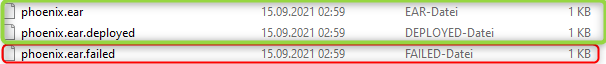
\includegraphics[width=1\linewidth]{source/general/deployments}
        \caption{Deployment-Status}
        \label{fig:deployment-status}
    \end{figure}
    Das entsprechende Mail ist im Anhang in folgendem Kapitel zu finden: \autoref{chap:811534244}
\end{flushleft}
\begin{flushleft}
    Allerdings ist dies nicht immer 100\% verlässlich.
    Die sicherste Methode, um die Funktionsfähigkeit eines Nodes resp.
    Servers zu testen besteht darin, die \textit{Workstation.exe} nur noch auf den entsprechenden Node resp.
    Server verbinden zu lassen.
    Die Verbindung wird ins \textit{Workstation.ini} geschrieben, welches wie üblich hier zu finden ist:
\end{flushleft}
\begin{flushleft}
    \dirtree{%
        .1 /.
        .2 C:\textbackslash.
        .3 Program Files (x86).
        .4 <Phoenix7-Verzeichnis>.
        .5 Workstation.ini.
    }
\end{flushleft}
\begin{flushleft}
    Im Ini stehen die \Gls{JBoss}-Server und Nodes im Eintrag \textit{-Dphoenix.server.nodes}.
    Hier das Beispiel des Produktiven Ini-Files:
    \lstset{style=gra_codestyle}
    \begin{lstlisting}[language=sh, caption=Workstation.ini PROD Beispiel,captionpos=b,label={lst:workstation.ini-prod-beispiel},breaklines=true]
    -clean
    -data
    @noDefault
    -configuration c:/temp/phoenix/prod_7_23_1/eclipse/configuration
    -nl
    de_CH
    -vmargs
    -Dorg.eclipse.update.reconcile=false
    -Dphoenix.db=Phoenix
    -Dphoenix.application.workspace.createdir=true
    -Dphoenix.application.workspace=\\\\phoenix\workspace\prod_7_23_1
    -Dphoenix.login.usernamefile=%APPDATA%/Phoenix/login_username_prod
    -Dphoenix.server.nodes=sks0020:8443,sks0021:8443,sks0020:8543,sks0021:8543
    -Djavax.net.ssl.trustStore=C:\Program Files (x86)\Phoenix7\truststore.jks
    -Dphoenix.login.enableLDAP=true
    -Dphoenix.application.winlogin=true
    -XX:-CreateMinidumpOnCrash
    \end{lstlisting}
\end{flushleft}
\begin{flushleft}
    Erkennen, ob ein \Gls{JBoss}-Service gestoppt ist, tut man daran, dass folgender Eintrag zuletzt im \texttt{server.log} steht:
    \lstset{style=gra_codestyle}
    \begin{lstlisting}[language=sh, caption=Service gestoppt - server.log,captionpos=b,label={lst:service-stopped-service.log},breaklines=true]
2024-01-05 10:56:10,422 INFO  [--] [org.jboss.as] ip[] mib[] user[] session[] request[] thread[MSC service thread 1-3]: WFLYSRV0050: JBoss EAP 7.4.8.GA (WildFly Core 15.0.19.Final-redhat-00001) stopped in 1199ms
    \end{lstlisting}
    Ein Erfolgreicher start erkennt man wiederum an folgenden Eintrag:
    \lstset{style=gra_codestyle}
    \begin{lstlisting}[language=sh, caption=Service gestartet - server.log,captionpos=b,label={lst:service-started-service.log},breaklines=true]
2024-01-05 11:01:36,000 INFO  [--] [com.cgm.phoenix.common.masterdata.srv.catalog.dao.CatalogValueDAO] ip[] mib[] user[] session[] request[] thread[ServerService Thread Pool -- 273]: Creating folder index...
2024-01-05 11:01:36,047 INFO  [--] [com.cgm.phoenix.common.masterdata.srv.catalog.dao.CatalogValueDAO] ip[] mib[] user[] session[] request[] thread[ServerService Thread Pool -- 273]: Creating search index...
2024-01-05 11:02:00,656 INFO  [--] [com.cgm.phoenix.common.masterdata.srv.catalog.dao.CatalogValueDAO] ip[] mib[] user[] session[] request[] thread[ServerService Thread Pool -- 273]: Catalog data loaded.
2024-01-05 11:02:00,656 INFO  [--] [com.cgm.phoenix.common.masterdata.srv.catalog.CatalogCacheProvider] ip[] mib[] user[] session[] request[] thread[ServerService Thread Pool -- 273]: Instant Catalogs successfully initialized.
2024-01-05 11:02:00,891 INFO  [--] [org.jboss.as.server] ip[] mib[] user[] session[] request[] thread[ServerService Thread Pool -- 43]: WFLYSRV0010: Deployed "phoenix.ear" (runtime-name : "phoenix.ear")
2024-01-05 11:02:00,891 INFO  [--] [org.jboss.as.server] ip[] mib[] user[] session[] request[] thread[ServerService Thread Pool -- 43]: WFLYSRV0010: Deployed "jolokia.war" (runtime-name : "jolokia.war")
2024-01-05 11:02:00,922 INFO  [--] [org.jboss.as.server] ip[] mib[] user[] session[] request[] thread[Controller Boot Thread]: WFLYSRV0212: Resuming server
2024-01-05 11:02:01,000 INFO  [--] [org.jboss.as] ip[] mib[] user[] session[] request[] thread[Controller Boot Thread]: WFLYSRV0025: JBoss EAP 7.4.8.GA (WildFly Core 15.0.19.Final-redhat-00001) started in 281140ms - Started 18250 of 18473 services (563 services are lazy, passive or on-demand)
2024-01-05 11:02:01,000 INFO  [--] [org.jboss.as] ip[] mib[] user[] session[] request[] thread[Controller Boot Thread]: WFLYSRV0060: Http management interface listening on http://10.0.22.52:9990/management
2024-01-05 11:02:01,016 INFO  [--] [org.jboss.as] ip[] mib[] user[] session[] request[] thread[Controller Boot Thread]: WFLYSRV0051: Admin console listening on http://10.0.22.52:9990
    \end{lstlisting}

    Es kann aber mehrere Minuten dauern, bis ein Service vollständig gestartet ist.
\end{flushleft}
\begin{flushleft}
    Am Einfachsten ist, man erstellt sich drei Ini-Files, eines für beide Server zusammen im Cluster und eines pro Server.
    Dann braucht man nur die Files umzubennen und kann rasch Testen.
\end{flushleft}
\begin{flushleft}
    \begin{mdframed}
    Vorsichht!\\Es kann vorkommen, dass jeder Server für sich alleine Lauffähig ist aber im Cluster-Verbund keine Anmeldung möglich ist!\\
    Daher sollte nach einem Reboot nebst der Lauffähigkeit der einzelnen Nodes auch immer der Cluster getestet werden!
    \end{mdframed}
\end{flushleft}
\begin{flushleft}
    Obwohl die Server mittels \Gls{Ivanti} betankt werden, kann es vorkommen, dass nicht alle Patches geladen wurden.
    Um sicherzustellen, dass das System komplett sauber gepatched wurde, sollte man immer noch auf Updates Prüfen.

    Geprüft wird Normal via Suche:
    \begin{figure}[H]
        \centering
        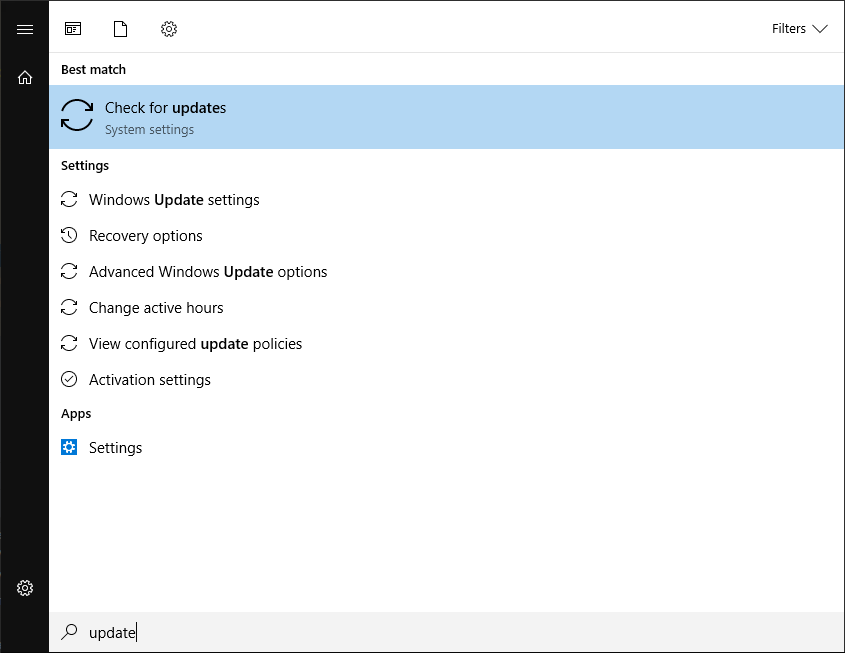
\includegraphics[width=1\linewidth]{source/general/search_for_updates}
        \caption{Check-Updates}
        \label{fig:check-updates}
    \end{figure}

    \begin{mdframed}
    Wurde der Server von Ivanti korrekt betankt, so sind meistens zwei Patches vorhanden bei denen \texttt{Restart required} steht.
    \end{mdframed}

    Solange noch Updates wie folgt, vorhanden sind, müssen diese manuell nachgeladen und installiert werden:
    \begin{figure}[H]
        \centering
        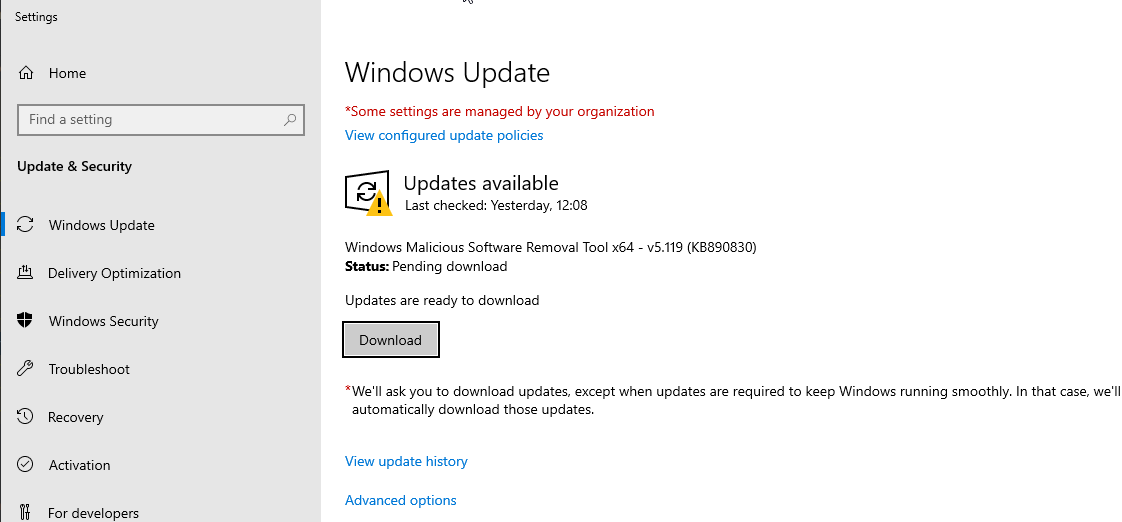
\includegraphics[width=1\linewidth]{source/general/updates_available}
        \caption{Updates available}
        \label{fig:updates-available}
    \end{figure}

    Dies ist aber äusserst selten der Fall.

    \begin{mdframed}
    Vorsichht!\\Sollte es trotzdem mal vorkommen, niemals die \Gls{RDP}-Verbindung schliessen!\\Ansonsten wird es unmöglich sein, den Server gezielt zu rebooten.
    \end{mdframed}
\end{flushleft}
\begin{flushleft}
    Desweiteren muss auf der \Gls{VMware vSphere} die Berechtigung gegeben sein, Snapshots erstellen und löschen zu können.
    Auch Restores via Snapshot sollten machbar sein.
\end{flushleft}
    %! Author = itgramic
%! Date = 24.11.23

% Preamble
\chapter{Testsystem}
\begin{flushleft}
    Beim
    \begin{figure}[H]
        \centering
        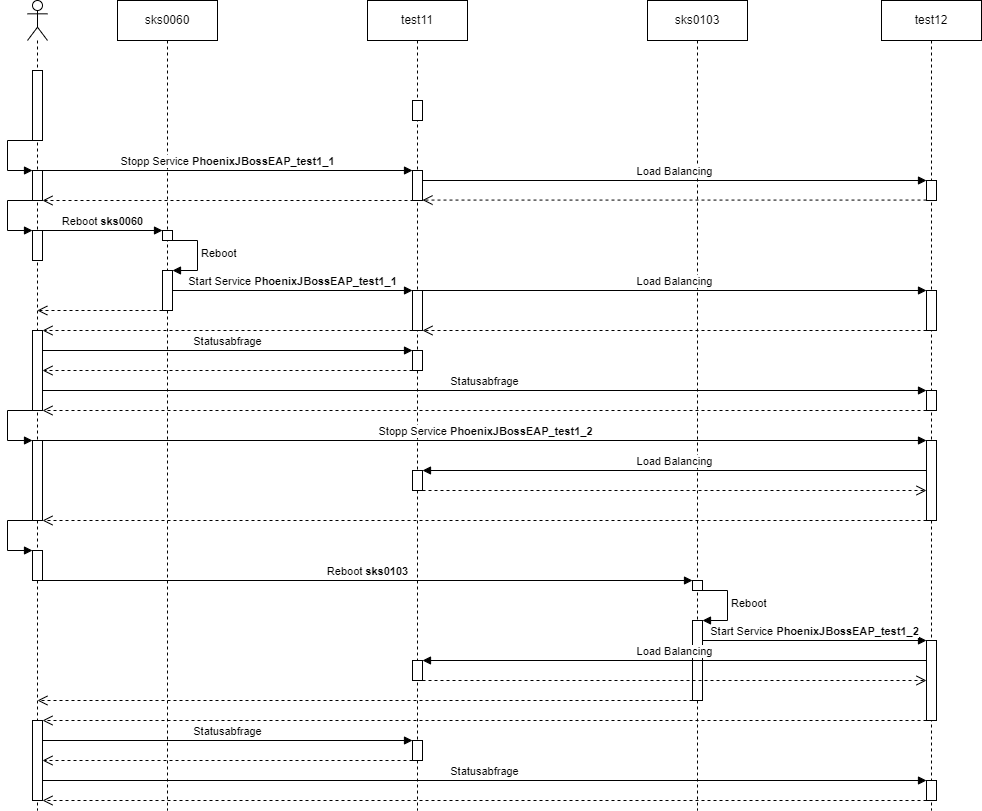
\includegraphics[width=1\linewidth]{source/test/sequenzdiagramm_test}
        \caption{TEST-Sequenzdiagramm}
        \label{fig:test-sequenzdiagramm}
    \end{figure}
\end{flushleft}
    %! Author = itgramic
%! Date = 24.11.23

% Preamble
\chapter{Produktivsystem}
\begin{flushleft}
    Beim Produktivsystem
    \begin{figure}[H]
        \centering
        
\includegraphics[width=1\linewidth]{source/prod/sequenzdiagramm_prod}
        \caption{PROD-Sequenzdiagramm}
        \label{fig:prod-sequenzdiagramm}
    \end{figure}
\end{flushleft}
    %! Author = itgramic
%! Date = 09.01.24

% Preamble
\chapter{Snapshots}
{
    \begin{flushleft}
        Um Snapshots für die Server zu machen, muss in die \Gls{VMware vSphere} ESXi-Site geöffnet werden:
    \end{flushleft}
    \begin{flushleft}
        \url{https://sks0174.sivc.first-it.ch/ui/}
    \end{flushleft}
    \begin{flushleft}
        Dort muss dann der entsprechende Server, in diesem Beispiel \texttt{sks0060}, gesucht werden und auf \texttt{Snapshots} gewechselt werden:
        \begin{figure}[H]
            \centering
            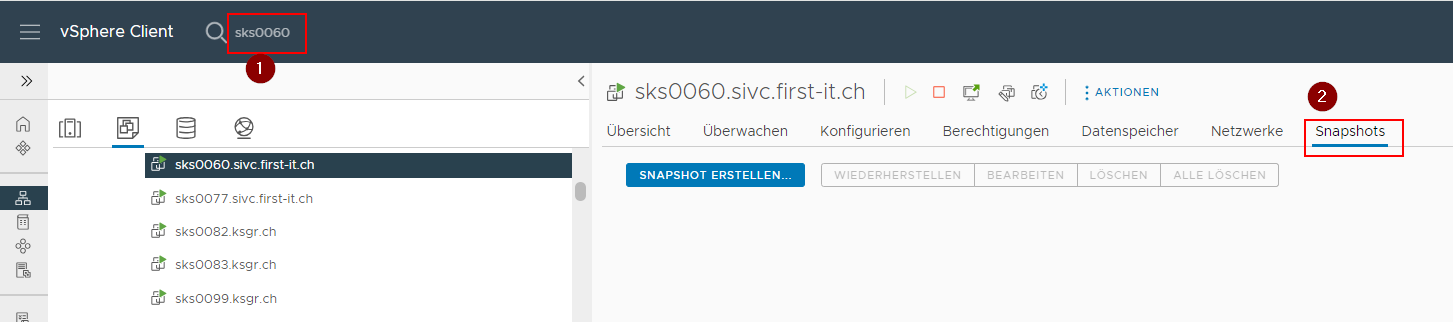
\includegraphics[width=1\linewidth]{source/snapshots/esxi_select_machine}
            \caption{ESXi - Maschine Suchen}
            \label{fig:esxi_select_machine}
        \end{figure}
    \end{flushleft}
    \begin{flushleft}
        Jetzt muss \texttt{SNAPSHOT ERSTELLEN...} geklickt werden.
        Wichtig ist, einen sprechenden Text in die Beschreibung zu hinteregen.
        \begin{figure}[H]
            \centering
            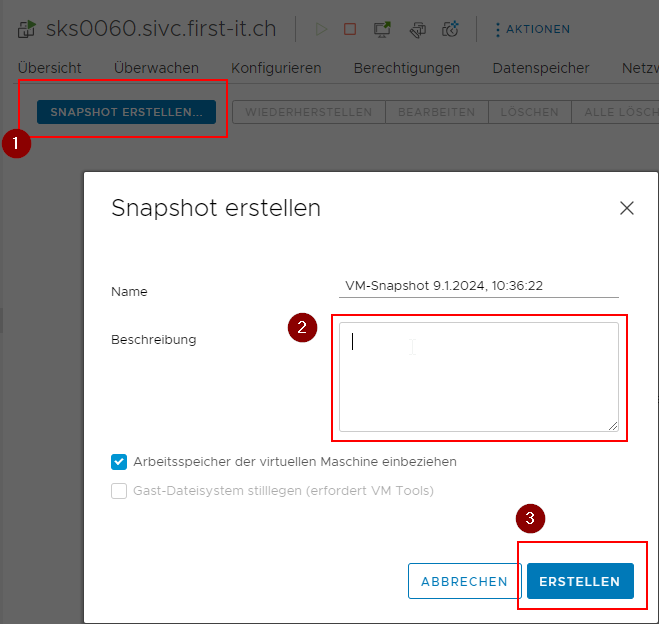
\includegraphics[width=0.5\linewidth]{source/snapshots/esxi_set_snapshot}
            \caption{ESXi - Snapshot erstellen}
            \label{fig:esxi_set_snapshot}
        \end{figure}
    \end{flushleft}
    \begin{flushleft}
        Die erstellung eines Snapshots kann bis zu meheren Minuten dauern.
        \begin{figure}[H]
            \centering
            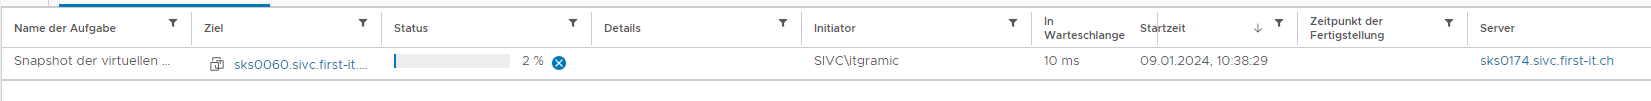
\includegraphics[width=1\linewidth]{source/snapshots/esxi_create_snapshote}
            \caption{ESXi - Snapshot wird erstellt}
            \label{fig:esxi_create_snapshote}
        \end{figure}
    \end{flushleft}
    \begin{flushleft}
        Ist der Snapshot erstellt, wird dies rückgemeldet:
        \begin{figure}[H]
            \centering
            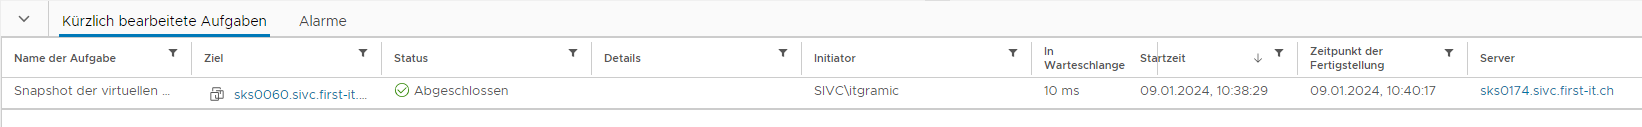
\includegraphics[width=1\linewidth]{source/snapshots/esxi_snapshot_created}
            \caption{ESXi - Snapshot wurde erstellt}
            \label{fig:esxi_snapshot_created}
        \end{figure}
    \end{flushleft}
}
{
    \begin{flushleft}
        Um einen Snapshot zu löschen, muss dieser ganz einfach angewählt werden\\
        und dann auf \texttt{LÖSCHEN} geklickt werden, wenn man nur einen Snapshot löschen will,
        \\oder \texttt{ALLE LÖSCHEN} wenn man alle Snpashots löschen will:
        \begin{figure}[H]
            \centering
            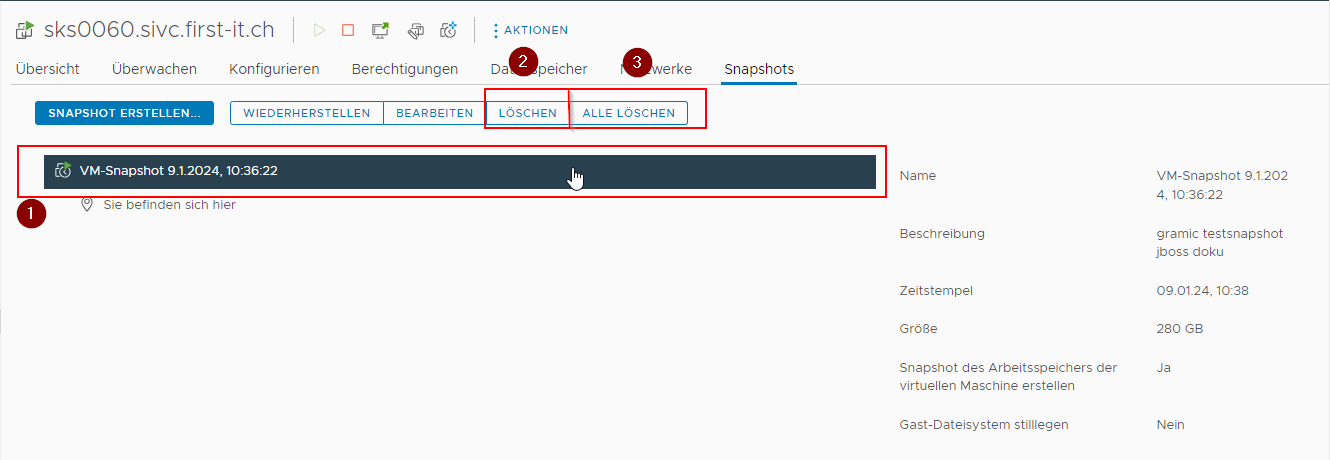
\includegraphics[width=0.5\linewidth]{source/snapshots/esxi_delete_snapshot}
            \caption{ESXi - Snapshot löschen}
            \label{fig:esxi_delete_snapshot}
        \end{figure}
    \end{flushleft}
    \begin{flushleft}
        Man muss aber bestätigen, dass man löschen möchte:
        \begin{figure}[H]
            \centering
            
\includegraphics[width=0.5\linewidth]{source/snapshots/esxi_confirm_delete}
            \caption{ESXi - Snapshot löschen bestätigen}
            \label{fig:esxi_confirm_delete}
        \end{figure}
    \end{flushleft}
    \begin{flushleft}
        Auch das löschen kann eine weile dauern.
        Wurde der Snapshot gelöscht, wird auch das zurückgemeldet:
        \begin{figure}[H]
            \centering
            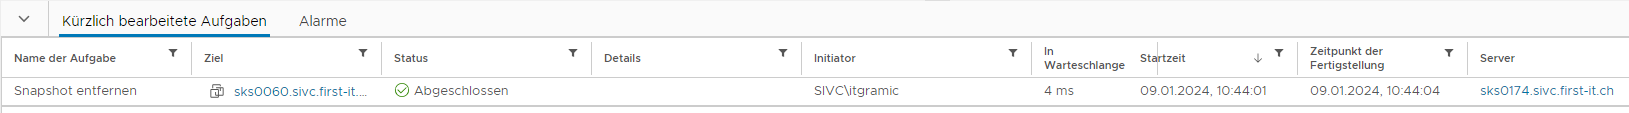
\includegraphics[width=0.5\linewidth]{source/snapshots/esxi_snapshot_deleted}
            \caption{ESXi - Snapshot gelöscht}
            \label{fig:esxi_snapshot_deleted}
        \end{figure}
    \end{flushleft}
    \begin{flushleft}
        \begin{mdframed}
            Bitte Snapshots Zeitnah löschen!\\
            Für längere Sicherungen ist das \Gls{VEEAM}-Backup vorhanden.\\
            Wird der Snapshot für länger als 3 Tage nicht gelöscht, so wird eine Meldung via Mail gesendet.
        \end{mdframed}
    \end{flushleft}
}
    %! Author = itgramic
%! Date = 11.10.23

% Preamble
%\begin{flushleft}
{
    \hypersetup{hidelinks}
    \listoffigures
}
%\end{flushleft}

\pagestyle{headings}
\thispagestyle{fancy}
%\begin{flushleft}
{
    \hypersetup{hidelinks}
    \listoftables
    \thispagestyle{fancy}
}
%\end{flushleft}
\pagestyle{headings}
\thispagestyle{fancy}

%\begin{flushleft}
{
    \cleardoublepage
    \renewcommand{\bibsetup}{\thispagestyle{fancy}}

    \printbibliography
}
%\end{flushleft}
%\begin{flushleft}
{
    \renewcommand*\glossarypreamble{\thispagestyle{fancy}}
    \printnoidxglossaries
}
%\end{flushleft}

\end{document}